\chapter{Introduction à l'apprentissage profond}\label{chap:intro ml}

L'astronomie, l'astrophysique et la cosmologie sont officiellement entrées dans l'ère du \textit{Big Data}, 
soit une ère dominée par le volume de données, maintenant mesuré dans l'ordre du \textit{petabyte}. Un \textit{petabyte} représente 
un million de \textit{gigabytes}, ou encore $\sim 10^{15}$ \textit{bytes}. 
En exemple particulier est l'observatoire Vera C. Rubin. Cet observatoire produira environ 1 \textit{petabytes} de données chaque année, soit une quantité de données 
impossible à traiter dans son ensemble pour la plupart des algorithmes; 
sans parler de la quantité accumulée par l'observatoire au travers des 10 années planifiées pour le relevé astronomique qui doit débuter 
en $2024$ \citep{lsst2009,lsst2021}. 

C'est cette réalité qui nous force à développer des méthodes d'analyses plus sophistiquées pour l'inférence de quantités physiques à partir 
d'images, spectres et vidéos du ciel. C'est aussi ce qui motive l'étude des méthodes liées à l'apprentissage machine, et plus particulièrement 
l'apprentissage profond, qui promettent de simplifier énormément l'analyse statistique des grands ensembles de données à venir. Ce chapitre se veut 
une courte introduction aux concepts de base. 
La section \ref{sec:bayes} est un survol de la théorie des statistiques bayésiennes. Cette section introduit certains concepts cruciaux qui sous-tendent la 
théorie de l'apprentissage machine. Ensuite, la section \ref{sec:app classique} décrit en détail un exemple de régression, 
puis la section \ref{sec:selection modele} discute du problème de la sélection du modèle.
Les réseaux neuronaux et l'apprentissage profond sont introduits à la section \ref{sec:app profond} 
comme une généralisation possible de l'apprentissage machine classique. Finalement, on introduit les 
réseaux de neurones convolutifs à la section \ref{sec:cnn}, cruciaux pour le traitement d'images.

Pour une discussion plus détaillée des concepts abordés dans ce chapitre, voir les manuels de référence \citet{Goodfellow2016} et \citet{Bishop2007}.

\section{Survol des statistiques bayésiennes}\label{sec:bayes}

L'inférence bayésienne est une théorie statistique qui a pour but principal de modéliser l'état de connaissance, 
ou le degré de croyance, associé à un évènement. De façon générale, l'inférence bayésienne est un processus de mise à jour de nos 
connaissances \textit{a priori}, c.-à-d. les connaissances acquises avant l'observation d'un évènement. 
On définit la vraisemblance comme la loi de probabilité qui gouverne la probabilité d'observer un évènement particulier.
Étant donné un processus physique auquel on associe une loi de vraisemblance, le processus d'inférence 
bayésienne correspond simplement à la repondération de nos connaissances par la vraisemblance. 
En d'autres mots, cette procédure correspond à multiplier la loi de probabilité \textit{a priori} par la vraisemblance d'un évènement (et renormaliser).

Par exemple, considérons un tirage au sort. 
On modélise la probabilité, $x \in [0, 1]$, d'observer pile ou face, $y \in \{0, 1\}$, 
par une loi de Bernoulli 
\begin{equation}
        p(y \mid x) = x^{y} (1 - x)^{1 - y}\, .
\end{equation} 
\textit{A priori}, on associe une probabilité égale (uniforme) au paramètre $x$, soit $p(x) = \mathcal{U}(0, 1)$. 
Ce choix reflète une ignorance complète du processus physique qui contrôle le tirage au sort.
Supposons maintenant qu'on observe $y_1$, un évènement généré de la loi physique $p(y_1 \mid x^{\star})$, où $x^{\star}$ est le véritable paramètre de la loi physique.
Le théorème de Bayes nous indique comment ajuster notre degré de croyance, maintenant $p(x \mid y_1)$, soit la loi \textit{a posteriori} du paramètre $x$ étant donné avoir observé $y_1$
\begin{equation}\label{eq:Bayes1}
        p(x \mid y_1) = \frac{p(y_1 \mid x) p(x)}{p(y_1)} \, .
\end{equation} 
La loi de probabilité $p(y)$, aussi appelée l'évidence, normalise la loi \textit{a posteriori}, qui est proportionnelle au produit de la vraisemblance $p(y \mid x)$ et 
de la loi \textit{a priori} $p(x)$. En pratique, on peut évaluer $p(y)$, une loi marginale, en l'exprimant 
en fonction de la loi jointe $p(x, y)$, soit 
\begin{equation}
        p(y) = \int_\mathcal{X} dx\, p(y, x) \, .
\end{equation} 
On peut ensuite utiliser la définition d'une loi conditionnelle 
\begin{equation}
        p(y \mid x) = \frac{p(x,\, y)}{p(x)} \, ,
\end{equation} 
pour exprimer l'évidence, $p(y)$, en fonction de la vraisemblance et de la loi \textit{a priori} 
\begin{equation}
        p(x \mid y) = \frac{p(y \mid x) p(x)}{\int_\mathcal{X} dx\, p(y \mid x) p(x)} \, .
\end{equation} 
Supposons maintenant qu'on observe un certain nombre de tirages au sorts supplémentaires
\begin{equation*}
        y_2,y_3\dots,y_N \overset{\mathrm{iid}}{\sim} p(y \mid x^{\star})\, ,
\end{equation*}
indépendamment et identiquement distribués (iid) selon la même loi physique, $p(y \mid x^{\star})$. Pour mettre à jour nos connaissances, on procède 
itérativement. En premier lieu, on trouve la distribution \textit{a posteriori} $p(x \mid y_1)$ avec le théorème de Bayes \eqref{eq:Bayes1}. Ensuite, 
on remplace la distribution \textit{a priori}, $p(x)$, par $p(x \mid y_1)$ et on remplace la loi de vraisemblance par $p(y_2 \mid x)$ dans le théorème de Bayes \eqref{eq:Bayes1} 
pour obtenir la loi \textit{a posteriori}, $p(x \mid y_1, y_2)$. Et ainsi de suite.
Puisque les observations sont iid, alors ce processus est équivalent, par induction, à 
\begin{equation}\label{eq:BayesN}
        p(x \mid y_{1:N}) = \frac{\prod_{i=1}^{N} p(y_i \mid x) p(x)}{\int_\mathcal{X} \prod_{i=1}^{N}p(y_{i} \mid x) p(x) dx}
\end{equation} 
Ce dernier résultat est particulièrement important pour l'inférence statistique et la dérivation des fonctions 
objectives pour l'apprentissage machine. La figure \ref{fig:bayes update} montre comment nos connaissances 
sur le paramètre $x$ évoluent en termes du nombre d'observations effectuées lorsqu'on applique l'équation \eqref{eq:BayesN}. 
La figure montre que la loi \textit{a posteriori} correspond à la loi \textit{a priori} lorsque $N = 0$ 
et converge vers une loi normale centrée autour de $x^{\star}=\frac{1}{2}$ lorsque $N \rightarrow \infty$, 
soit un exemple concret du théorème de la limite centrale.
\begin{figure}[H]
        \centering
        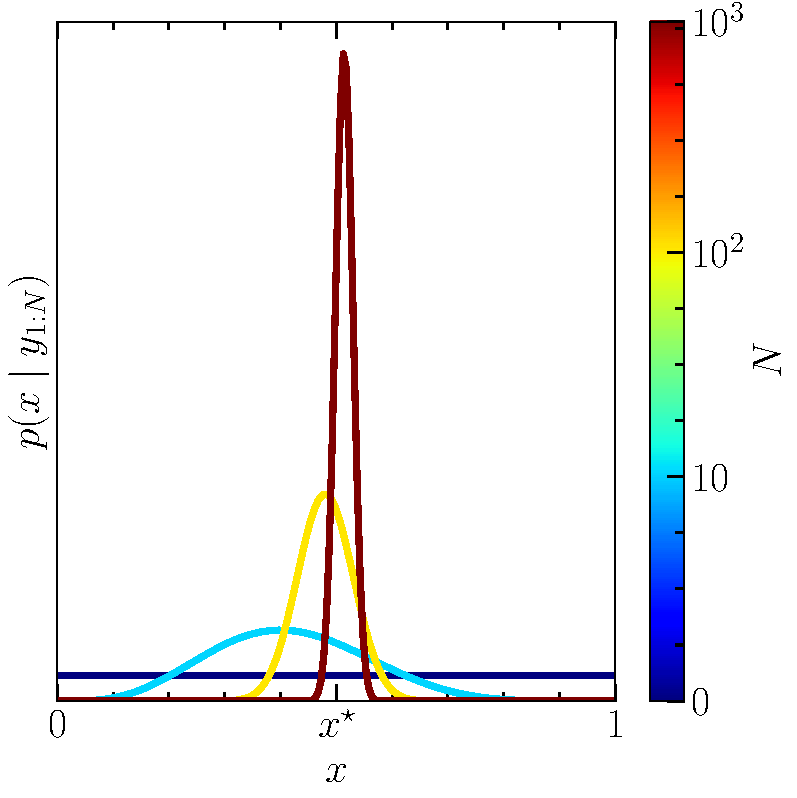
\includegraphics[width=0.4\textwidth]{notebooks/toy_coin_toss.pdf}
        \caption{Exemple d'une inférence bayésienne pour le tirage au sort.}
        \label{fig:bayes update}
\end{figure}

Le lecteur aura compris qu'on va maintenant construire l'apprentissage machine sur des fondations bayésiennes. Ce n'est pas la seule façon de le 
faire. En particulier, il est possible de poser des fondations fréquentistes en supposant, comme fait dans cette section, que toute l'information 
concernant un problème est contenue dans la loi de vraisemblance. Autrement dit, on suppose une ignorance complète \textit{a priori} sur les paramètres d'intérêts. 
En ce sens, et strictement dans le contexte qui nous intéresse, il est possible de passer d'un point de vue à l'autre, puisque les deux théories seront en accord 
sur la réponse à condition qu'on utilise une loi uniforme pour représenter nos connaissances \textit{a priori} sur les paramètres d'intérêts. 
À cause de cette correspondance approximative entre les deux théories, les lois 
\textit{a priori} vont parfois être abandonnées sans justification dans le texte qui suit. 
Le lecteur comprendra qu'on aura simplement changé de point de vue. 

\section{Un exemple d'apprentissage machine: la régression}\label{sec:app classique}

L'apprentissage machine est un concept assez général qui décrit le processus d'extraire l'information contenue 
dans un ensemble de données $\mathcal{D} = \{y_i\}_{i=1}^{N}$, soit un ensemble d'observations provenant d'une source ou d'un processus 
physique quelconque. Le terme \textit{information} est utilisé de façon très vague ici. Ce terme est formellement défini dans la théorie 
de l'information de \citet{Shannon1948} comme étant le nombre minimal de \textit{bits} pour décrire une observation $y_i$, ou encore 
l'ensemble de données $\mathcal{D}$. Cette quantité est intimement liée avec l'entropie. Une discussion plus détaillée est 
repoussée au chapitre \ref{chap:intro ml 2}.

Il y a quatre ingrédients essentiels à l'apprentissage machine, soit
\begin{enumerate}
        \item Un ensemble de données $\mathcal{D}$
        \item Un ensemble d'hypothèses $\mathcal{H}$
        \item Une fonction objective $\mathcal{L}$
        \item Un algorithme d'optimisation $\mathcal{G}$
\end{enumerate}
Dans cette section, je décris chacun de ces ingrédients dans le contexte d'une tâche de régression.
La régression est une tâche d'apprentissage machine qui consiste à entraîner un modèle, $f_{\theta}$, sur un ensemble de données augmenté pour la régression, soit 
$\mathcal{D} = \{(x_i, y_i)\}_{i=1}^N$. Chaque exemple dans l'ensemble de données est constitué d'un paramètre physique, $x$, et d'une observation, $y$. 
On suppose toujours que les exemples de l'ensemble de données sont générés de façon identique et indépendante par la combinaison 
d'une loi \textit{a priori} sur les paramètres physiques et une loi de vraisemblance pour les observations
\begin{equation}
                x \sim p(x),  \hspace{1cm} y\ \sim p_\theta(y \mid x) \, . 
\end{equation}
Dans le texte, on utilisera le terme \textit{modèle physique} pour faire référence à $p_\theta(y \mid x)$, puisque cette loi de probabilité relie les paramètres physiques, $x$, 
avec les observations, $y$. Elle encodera donc tous les processus physiques en jeu pour un problème d'inférence donné.
On notera de plus que l'ensemble des points de données n'a pas besoin d'être un nombre fini. Dans le cas où $N \rightarrow  \infty$, alors 
$\mathcal{D}$ est explicitement décrit par la loi \textit{a priori}, $p(x)$, et le modèle physique $p_\theta(y \mid x)$. 
Dans ce cas, on dira que la loi générative $(x, y) \sim p(x, y)$ est explicite. 
Dans le cas où $\mathcal{D}$ est un nuage de points avec $N < \infty$, alors on dira que le processus génératif est implicite. 

Pour se fixer les idées, on considère l'exemple  
\begin{equation}\label{eq:loi generative}
        p(x) = \mathcal{U}(a, b), \hspace{1cm} p_\theta(y \mid x) = \mathcal{N}(y \mid f_\theta(x), \sigma^2)\, .
\end{equation}
On a utilisé le symbole $\mathcal{N}(y \mid \mu, \sigma^2)$ pour décrire une loi normale sur $y$ avec comme moyenne $\mu$ et variance $\sigma^2$. 
On doit supposer que les données sont générées à partir d'une solution quelconque 
\begin{equation}
        f_{\theta^{\star}} = 2x^5 - x\, ,
\end{equation}
avec une amplitude de bruit $\sigma=1$. Ce problème est illustré à la figure \ref{fig:toy problem}.
\begin{figure}[th!]
        \centering
        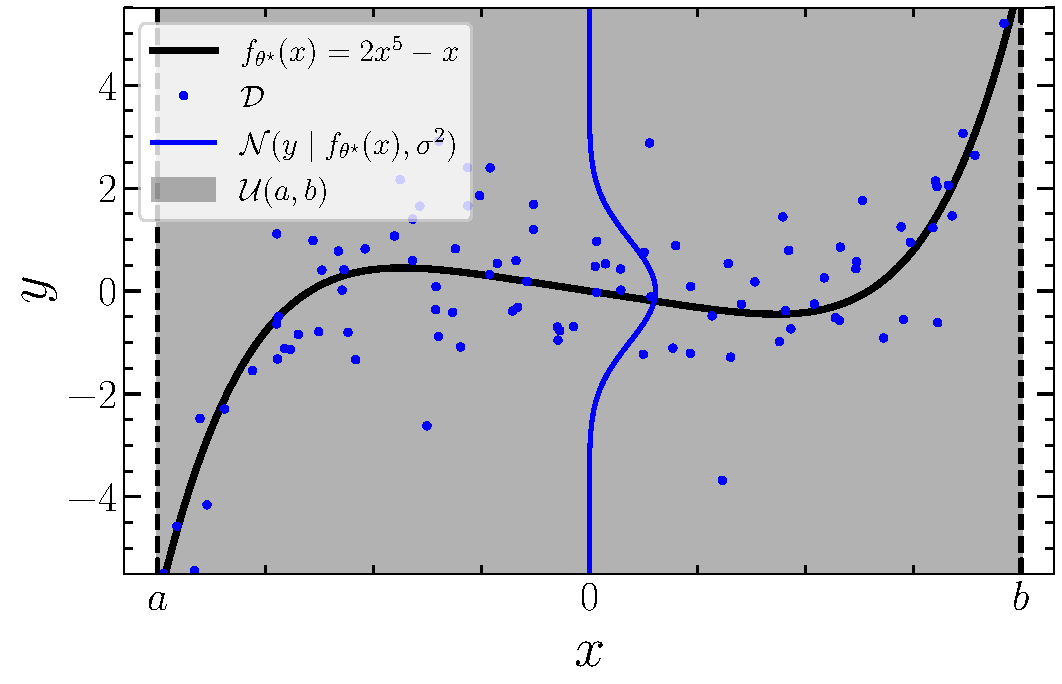
\includegraphics[width=0.5\textwidth]{notebooks/toy_problem}
        \caption{Exemple d'un problème de régression.}
        \label{fig:toy problem}
\end{figure}

Le second ingrédient au problème d'apprentissage machine est la famille des modèles, ou l'ensemble des hypothèses, $\mathcal{H}$. 
Il serait tentant de choisir le modèle $f_\theta = \theta_1 x^{5} + \theta_2 x$, soit un modèle avec la même forme que la solution 
$f_{\theta^{\star}}$. Toutefois, on ne peut pas assumer que la forme du modèle sera connue \textit{a priori}, 
ou qu'elle peut facilement être devinée. La sélection du modèle sera abordée en détail dans la section \ref{sec:selection modele}, 
puisque ce sujet mérite une discussion à part entière.
Pour l'instant, on va simplement faire le choix le plus simple en assumant que la forme de 
la loi utilisée pour générer les points de données est inconnue. 
Le choix le plus simple est de construire une famille de modèles linéaires en termes de $x$ et $\theta$
\begin{equation}\label{eq:modele lineaire}
        \mathcal{H} = \{f_\theta:\mathbb{R} \rightarrow  \mathbb{R} \mid f_\theta = \theta_0 + \theta_1 x\}\, . 
\end{equation} 
Le troisième ingrédient à l'apprentissage machine est de construire une fonction objective pour \textit{entrainer} notre modèle $f_\theta$ sur les points 
de données observés. 
L'objectif de l'entraînement est d'estimer le modèle $f_\theta$, ou de façon équivalente les paramètres $\theta$, qui maximise la loi \textit{a posteriori}, $p(\theta | \mathcal{D})$. En appliquant 
le théorème de Bayes, ceci correspond à
\begin{equation}
        \hat{\theta} = \underset{f_\theta \in \mathcal{H}_\theta}{\mathrm{arg\, max}}\, \frac{p(\mathcal{D} \mid \theta) p(\theta)}{p(\mathcal{D})}
\end{equation} 
Pour faire correspondre cet objectif avec la littérature, on applique le logarithme au côté droit de l'équation, ce qui ne change pas la position des extremas de 
l'objectif, le logarithme étant une fonction monotone. Il est aussi convention de tourner le problème à l'envers, et de chercher plutôt les minimas de la fonction négative. Dans 
ce cas, la fonction objective est
\begin{equation}
        \hat{\theta} = \underset{f_\theta \in \mathcal{H}}{\mathrm{arg\, min}}\, -\log p(\mathcal{D} \mid \theta) - \log p(\theta) + C(\mathcal{D})\, .
\end{equation} 
où $C(\mathcal{D})$ est une constante qui ne dépend que de l'ensemble de données. L'étape finale est d'écrire la vraisemblance $p(\mathcal{D} \mid \theta)$ 
en termes de $p_\theta( y \mid x)$. Dans le texte, les paramètres d'entraînements sont toujours placés en indices, 
par quoi on entend que les paramètres $\theta$ conditionnent la loi de probabilité, $p_\theta(x \mid y) = p(x \mid y, \theta)$. On remarque que
\begin{equation}
        p(\mathcal{D} \mid \theta) = \prod_{i=1}^{N}p(x_i, y_i \mid \theta) = \prod_{i=1}^{N}p(y_i \mid x_i, \theta) p(x_i \mid \theta)\, ,
\end{equation} 
par définition de la loi conditionnelle et de la supposition que les données sont générées de façon iid. 
Le dernier terme peut être simplifié en termes de la loi \textit{a priori}, $p(x \mid \theta) = p(x)$ 
puisqu'on suppose que $\theta$ et $x$ sont deux variables aléatoires indépendantes. Un choix de modèle $\theta$ ne devrait pas changer 
la distribution \textit{a priori} sur les paramètres physiques. Si c'est le cas, alors le choix du modèle doit être révisé.
On trouve finalement l'objectif d'entraîenement
\begin{equation}
        \hat{\theta} = \underset{f_\theta \in \mathcal{H}}{\mathrm{arg\, min}}\, -\prod_{i=1}^{N}\log p_\theta(y_i \mid x_i) - \log p(\theta) + C(\mathcal{D})\, ,
\end{equation} 
où $-\prod_{i=1}^N\log p(x_i)$ est absorbé dans $C(\mathcal{D})$. On est maintenant en mesure de dériver la forme exacte de la fonction objective pour le problème 
posé dans cette section. Avec la supposition que le modèle physique est une loi normale, on a que
\begin{equation}
       \log \prod_{i=1}^{N}p_\theta(y_i \mid x_i) = -\frac{1}{2}\sum_{i=1}^{N}\frac{(y_i - f_\theta(x_i))^2}{\sigma^2} - \frac{N}{2}\log(2\pi \sigma^2)\, ,
\end{equation} 
ce qui correspond à la fonction objective
\begin{equation}\label{eq:MSE intro}
        \hat{\theta} = \underset{f_\theta \in \mathcal{H}}{\mathrm{arg\, min}}\, \underbrace{ \frac{1}{N}\sum_{i=1}^{N}
        (y - f_\theta(x))^2 }_{\hat{\mathcal{L}}_\theta(\mathcal{D})}  - \frac{2\sigma^2}{N}\log p(\theta)\, .
\end{equation} 
Par convention, on a utilisé le fait que les constantes qui ne dépendent pas de $\theta$ peuvent être ignorées (elles ne changent pas les extremas du problème) 
et on a multiplié la fonction objective par $2\sigma^2 / N$. 
L'expression obtenue fait intervenir la fonction objective approximative $\hat{\mathcal{L}}_{\theta}(\mathcal{D})$, soit un estimé Monte Carlo de l'espérance de l'erreur 
quadratique. En prenant la limite $N \rightarrow \infty$, l'estimé Monte Carlo de l'espérance devient exacte
\begin{equation}
        \lim\limits_{N \rightarrow \infty}\hat{\mathcal{L}}(\mathcal{D}) = \mathcal{L}_{\theta}(\mathcal{D}) = \mathbb{E}_{(x, y) \sim \mathcal{D}} \big[(y - f_\theta(x))^2\big]\, .
\end{equation} 
Dans la littérature, $\hat{\mathcal{L}}_\theta(\mathcal{D})$ est nommée l'erreur quadratique moyenne. Dans le reste de ce mémoire, on va laisser 
tomber le chapeau sur la fonction objective pour simplifier la notation. Le lecteur comprendra qu'on travaille généralement avec l'estimé 
Monte Carlo si l'espérance mathématique n'est pas accessible par calcul direct.

Le dernier ingrédient à l'apprentissage machine est le choix d'un algorithme d'optimisation $\mathcal{G}$ pour résoudre l'équation \eqref{eq:MSE intro}, c.-à-d. déterminer 
$\hat{\theta}$. Les algorithmes d'optimisations récents pour l'apprentissage profond sont souvent basés sur la descente de gradient stochastique, qu'on peut décrire succinctement 
par la relation de récurrence
\begin{equation}\label{eq:gd}
        \hat{\theta}^{(t+1)} = \hat{\theta}^{(t)} - \gamma_t \grad_{\hat{\theta}^{(t)}} \mathcal{L}_{\hat{\theta}^{(t)}}(\mathcal{D})\, ,
\end{equation} 
$\gamma_t$ est le taux d'apprentissage, généralement choisi comme étant aussi grand que possible, 
sans pour autant rendre instable l'algorithme d'optimisation $\mathcal{G}$. Une discussion plus détaillée est reportée au chapitre \ref{chap:intro ml 2} sur ce sujet.

\begin{figure}[th!]
        \centering
        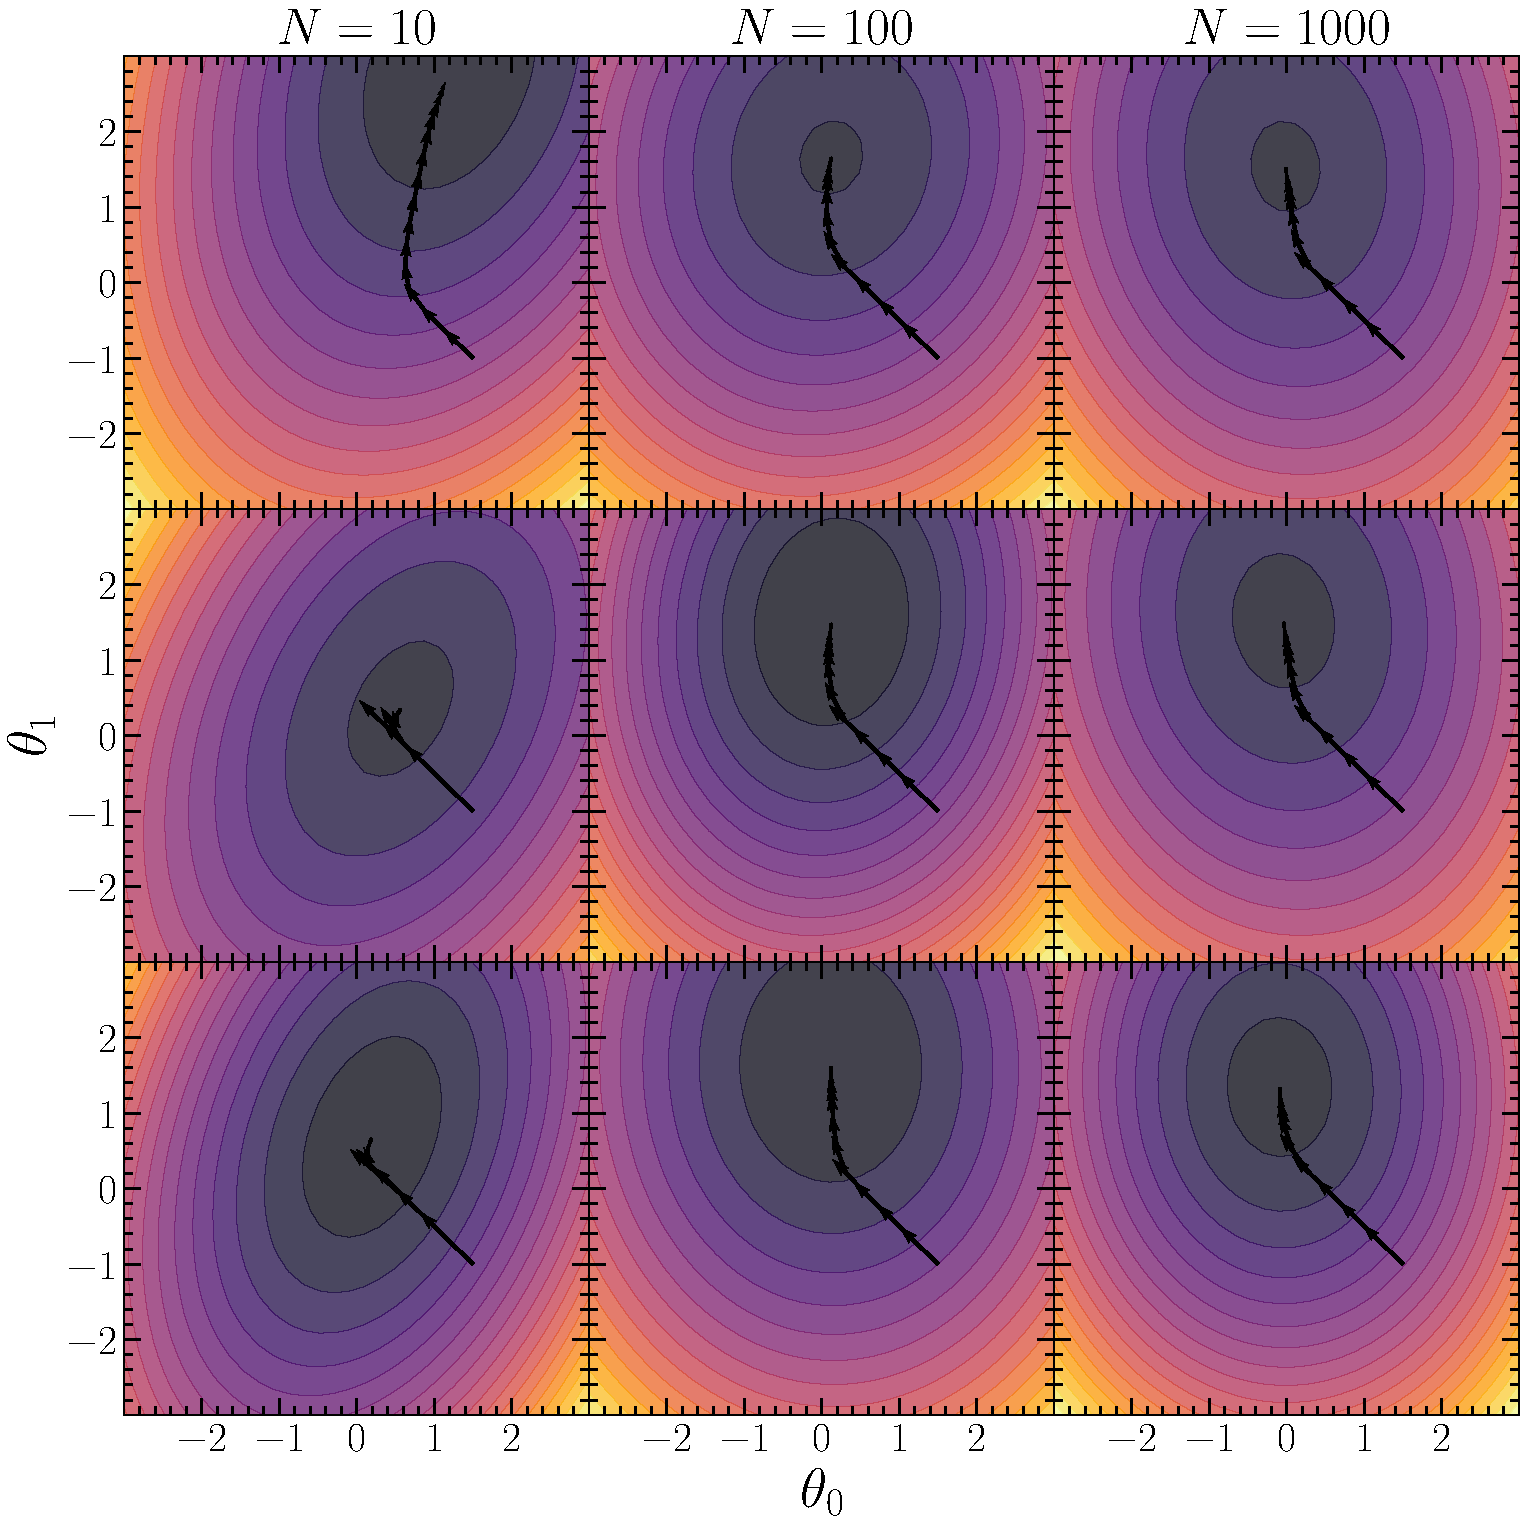
\includegraphics[width=0.7\textwidth]{notebooks/monte_carlo_loss.pdf}
        \caption{Contours de $\mathcal{L}_\theta(\mathcal{D})$ pour différent tirage de $\mathcal{D}$ (rangées) et différentes taille $N = |\mathcal{D}|$ (colonnes) 
                en utilisant le modèle linéaire de l'équation \eqref{eq:modele lineaire} et la loi générative \eqref{eq:loi generative}.
        Une trajectoire produite par la descente de gradient \eqref{eq:gd} est illustré avec les flèches noires.}
        \label{fig:monte carlo L}
\end{figure}

Lorsqu'on travaille à basses dimensions, il est possible d'obtenir de très bons estimés pour $\mathcal{L}_\theta(\mathcal{D})$. 
Par exemple, la figure \ref{fig:monte carlo L} illustre comment 
la variance des contours de l'estimé Monte Carlo $\mathcal{L}_{\theta}(\mathcal{D})$ diminue en fonction de $N$. 
Les rangées montrent un estimé Monte Carlo pour différents tirages de l'ensemble de données $\mathcal{D}$ à partir 
de la loi générative décrite à l'équation \eqref{eq:loi generative}, alors que les colonnes montrent  
des ensembles de données de taille croissante. En particulier, la troisième colonne possède des contours très stables, ce qui 
implique que la descente de gradient va retrouver la même solution $\hat{\theta}$ systématiquement, 
contrairement aux estimés où $N$ est relativement petit. Dans ce cas, la solution obtenue par $\mathcal{G}$ 
dépend fortement de l'ensemble de données observé; la première colonne est l'exemple le plus frappant de ce phénomène.


%Je termine cette courte introduction avec la définition de deux concepts qui portent parfois à confusion 
%dans le jargon de l'apprentissage profond, soit celui d'une \textit{batch} et d'une \textit{époque}.  
%Une \textit{batch} $\mathcal{B}$ est un sous ensemble de $\mathcal{D}$, soit $\mathcal{B} \subseteq \mathcal{D}$. Dans le même ordre d'idée du paragraphe précédent, les fonctions objectives 
%estimées à partir de différentes \textit{batch}, $\mathcal{L}(\mathcal{B})$, peuvent varier de manière significative entre chaque \textit{batch}. 
%Toutefois, sous certains conditions, une descente stochastique avec \textit{batch} est équivalente à une descente de gradient stoachastique avec $\mathcal{L}(\mathcal{D})$, 
%soit un estimé à partir de l'ensemble de donnée complet. La descente de gradient stochastique avec \textit{batch} 
%est donc particulièrement utile pour l'optimisation de modèles où les données traitées sont de très haute dimensions, 
%une situation où l'obtention de la quantité $\mathcal{L}(\mathcal{D})$ requiert souvent une quantité d'opérations machines prohibitive, contrairement à $\mathcal{L}(\mathcal{B})$.
%D'un autre côté, une \textit{époque} est un concept assez artificiel qui n'est pas réutilisé dans le reste de ce mémoire. Ce concept correspond à un 
%certains nombre d'itérations de la descente de gradient après lequel on aurait épuisé l'ensemble de donné, soit $T = \frac{|\mathcal{D}|}{|\mathcal{B}|}$, 
%en assumant que les \textit{batch} sont des sous ensembles distincts de $\mathcal{D}$. 

%Ceci complète donc cette introduction à l'apprentissage machine. 
Les quelques thèmes abordés ici seront suffisants
pour donner une compréhension à haut niveau des méthodes développées dans les prochains chapitres. Bien sûr, 
cette introduction n'est pas exhaustive. Un lecteur intéressé devrait consulter les références mentionnées au début du 
chapitre. Les sections qui suivent serviront à introduire et motiver l'apprentissage profond.


\section{Sélection du modèle}\label{sec:selection modele}

Pour motiver l'apprentissage profond, on s'intéresse maintenant au problème de la sélection du modèle. 
La sélection d'un modèle linéaire à la section précédente n'était motivée que par un critère de simplicité. En général, 
ce critère est insuffisant pour extraire toute l'information qu'un ensemble de données contient, et ce, peu importe les transformations appliquées 
aux espaces $\mathcal{X}$ et $\mathcal{Y}$. Par exemple, un polynôme avec un seul terme (monôme) comme $f_{\theta^{\star}}(x) = Cx^{\alpha}$ peut naturellement être modélisé 
par un modèle linéaire après la transformation appropriée de l'espace des paramètres physiques $\mathcal{X} \rightarrow  \log \mathcal{X}$, de sorte 
que le monôme dans le nouvel espace, $f'_{\theta^{\star}} = \alpha \log x + \log C$, est une fonction de forme linéaire en termes de $\alpha$, $\log C$ et $x$.
En général, le prétraitement des données est un aspect important de l'apprentissage machine puisqu'il permet d'éplucher les couches 
de complexités artificielles autour d'un problème d'apprentissage machine donné.

Or, la fonction introduite à la section précédente est déjà un exemple qui ne peut pas être recouvert par un modèle linéaire puisque 
$f_{\theta^{\star}} = 2x^{5} - x$ est un polynôme composé de deux monômes. Minimalement, deux modèles linéaires seraient donc nécessaires pour recouvrir $f_{\theta^{\star}}$.
Au mieux, un modèle linéaire est une bonne approximation de $f_{\theta^{\star}}$ pour des régions spéciales du domaine de la fonction comme $|x| \ll 1$ ou $|x| \gg 1$.
On doit donc considérer des modèles plus complexes que le simple modèle linéaire considéré jusqu'à maintenant.

Pour ce faire, on considère trois directions principales. 
La première méthode, déjà mentionnée dans la section précédente, est de construire une fonction avec la bonne forme \textit{a priori} via l'intuition.  
%ou possiblement plusieurs décennies de recherche pour les problèmes plus complexe. 
On ne considéra pas plus longtemps cette approche, puisqu'elle est impraticable dans les cas les plus généraux comme les problèmes à haute dimensions où l'intuition humaine échoue complètement.
La seconde approche, et probablement l'approche la plus intuitive considérant la façon dont le sujet a été introduit jusqu'à maintenant, est de considérer une série de puissances entières positives.
Puisque c'est une approche importante en apprentissage machine, il vaut la peine de dire quelques mots sur celle-ci avant de poursuivre vers la troisième 
et dernière approche possible. 

\subsection{Compromis entre le biais et la variance}
Lorsque $x \in \mathbb{R}$, la série entière prend la forme très simple
\begin{equation}\label{eq:power law}
        f_\theta(x) = \sum_{p = 0}^{P} \theta_p x^{p}\, .
\end{equation} 
%On notera $\mathcal{H}_P$ l'ensemble des polynômes de degré $P$ pour la discussion qui suit.
Le modèle \eqref{eq:power law} est une fonction linéaire en termes des paramètres $\theta$ et non-linéaire en termes des paramètres physiques $x$ ($P > 1$). 
Dans la limite où $P \rightarrow \infty$, ce modèle 
peut représenter l'ensemble des fonctions analytiques incluant les polynômes, $e^x$, les fonctions trigonométriques, hyperboliques, etc. 

Pour ce cas spécial, on peut explorer comment la complexité du modèle \eqref{eq:power law} influence le problème d'apprentissage. Strictement dans le contexte de l'ajustement 
d'un polynôme $f_\theta: \mathbb{R} \rightarrow \mathbb{R}$ de degré $P < \infty$, la complexité du modèle peut être quantifiée par $P$, soit le nombre de termes dans 
la série entière. En répétant l'exercice de la section précédente plusieurs fois pour des modèles d'une complexité grandissante,
on peut obtenir des statistiques sur l'erreur de généralisation en fonction de $P$, ce qui est illustré à la figure \ref{fig:bias_variance}.

L'erreur de généralisation est définie comme l'erreur quadratique moyenne d'une fonction calculée sur un ensemble test, distinct de l'ensemble d'entraînement 
utilisé pour ajuster la fonction.
Cette métrique permet d'estimer le risque encouru lorsqu'on tente d'utiliser une fonction au-delà de son ensemble d'entraînement.
On observe que notre estimé de l'erreur de généralisation atteinte un minimum à la complexité $P=5$, ce qui correspond au degré du polynôme objectif $f_{\theta^{\star}} = 2x^5 - x$. 

%definir erreur de généralisation
\begin{figure}[ht!]
        \centering
        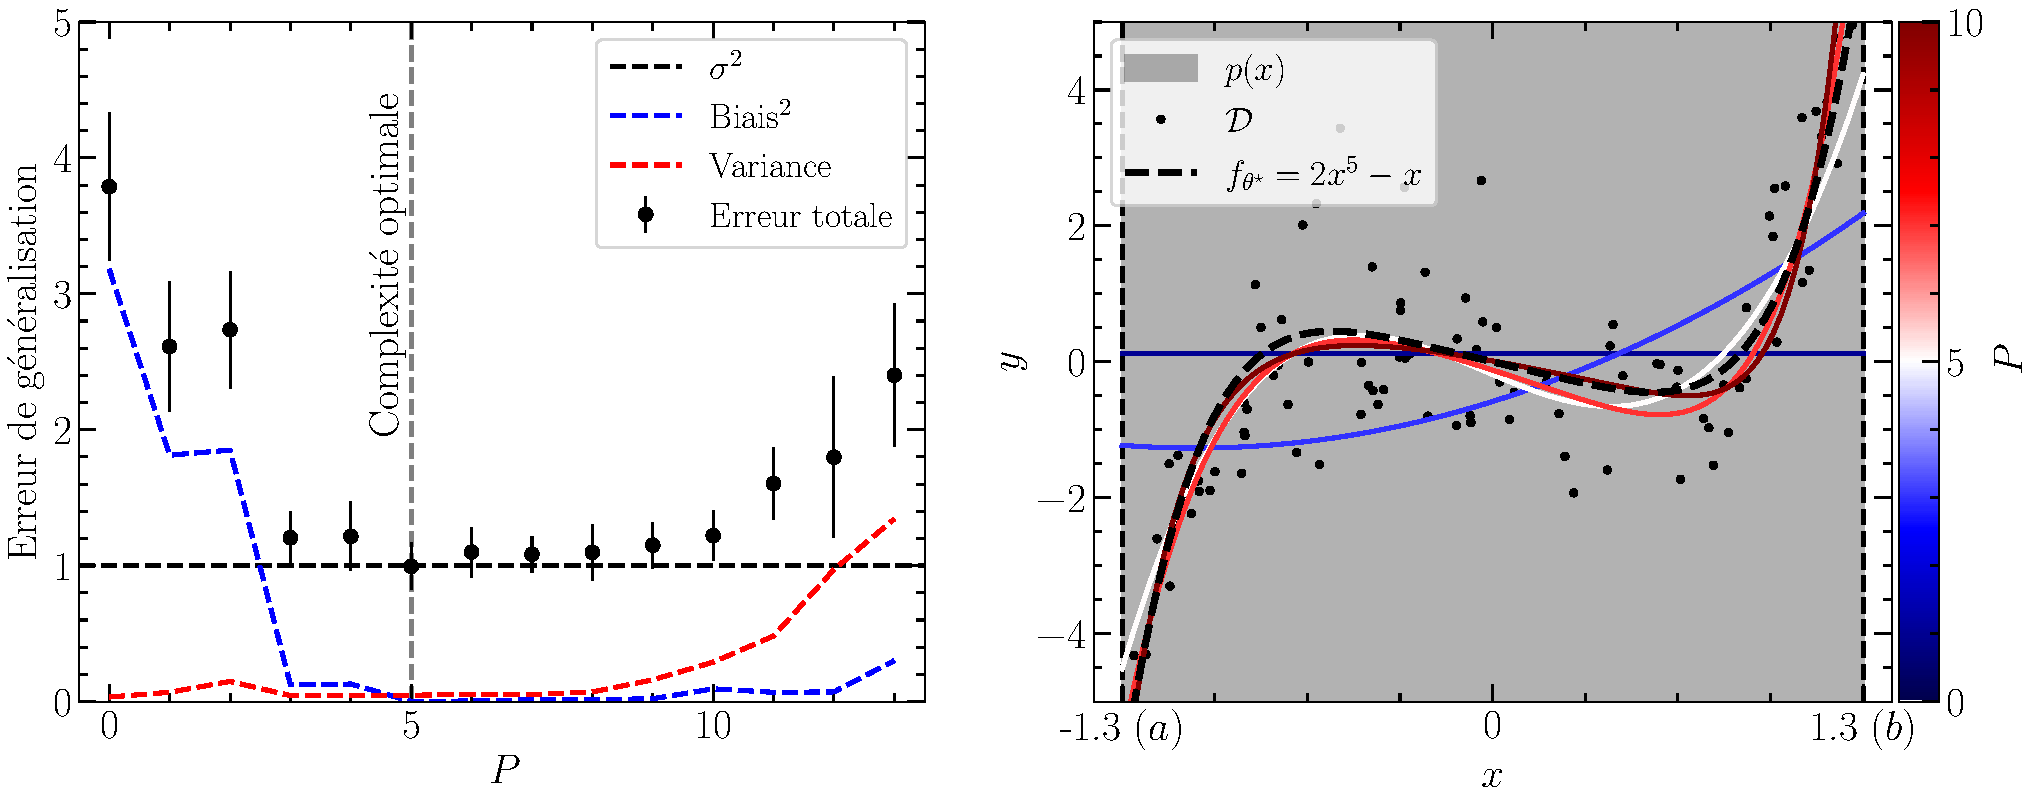
\includegraphics[width=\textwidth]{notebooks/bias_variance.pdf}
        \caption{Compromis classique entre le biais et la variance d'un algorithme d'apprentissage machine pour l'ajustement d'un polynôme de degré $P$ sur les données générées de la 
        loi $f_{\theta^\star} = 2x^5 - x$.}
        \label{fig:bias_variance}
\end{figure}

Le comportement de cette erreur 
peut être compris intuitivement par une décomposition de l'erreur totale en termes de l'erreur irréductible du problème 
$\sigma^2$, du biais 
\begin{equation}
        \mathrm{Biais}(f_{\theta}(x)) = \mathbb{E}_{\mathcal{D}}\left[ f_{\theta}(x)\right] - f_{\theta^{\star}}(x)\, ,
\end{equation} 
et de la variance d'un algorithme d'apprentissage machine 
\begin{equation}
       \mathrm{Variance}(f_\theta(x)) = \mathbb{E}_{\mathcal{D}}\left[ \big(f_{\theta}(x) - \mathbb{E}_{\mathcal{D}}\left[f_{\theta}(x) \right] \big)^2 \right]\, .
\end{equation} 
Lorsque le modèle n'est pas suffisamment complexe pour capturer l'ensemble des points de données, la solution est biaisée par le choix du modèle (courbes bleues de la 
figure \ref{fig:bias_variance}). Le biais est la principale cause du phénomène appelé le \textit{sous-ajustement}, soit lorsqu'un algorithme d'apprentissage n'est pas suffisamment 
flexible pour modéliser une certaine distribution $\mathcal{D}$. Lorsque le modèle est trop complexe, 
le modèle est aussi trop flexible et on observe un phénomène de \textit{sur-ajustement} (courbes rouges de la figure \ref{fig:bias_variance}). 
C.-à-d.~que les modèles entraînés se spécialisent à leur ensemble d'entraînement. 
L'erreur moyenne de généralisation augmente puisque la solution trouvée par l'algorithme d'apprentissage dépend fortement de l'ensemble d'entraînement $\mathcal{D}$, 
qui ne sera pas nécessairement représentatif de la loi générative implicite $f_{\theta^{\star}}(x)$. La variance domine l'erreur 
de généralisation dans ce régime.

Dans tous les cas, l'erreur minimale correspond à $\sigma^2$, soit le niveau d'erreur irréductible à un problème donné. 
Ce niveau d'erreur ne peut être atteint que lorsque la complexité du modèle est environ égale à la complexité de la loi 
générative. En général, on s'attend donc à ce qu'un niveau de complexité optimal existe pour un problème donné. 
La décomposition de l'erreur en termes du biais et de la variance est une méthode pour découvrir cette complexité. 
Cette procédure fonctionne certainement pour le problème de régression décrit dans cette section, mais elle n'est pas garantie de fonctionner en général. 
En effet, le biais et la variance d'une fonction sont des quantités presque impossibles à calculer en général, puisqu'on doit calculer l'espérance d'une fonction 
apprise par $\mathcal{G}$ étant donné différentes réalisations de $\mathcal{D}$.

Ce qui nous concerne maintenant est une discussion sur la sélection du modèle lorsqu'on doit apprendre 
une fonction sur des données multidimensionnelles, soit le cas plus général d'apprentissage machine.


\subsection{La séparabilité linéaire}
C'est lorsqu'on cherche à construire une série entière pour des données multidimensionnelles qu'on réalise que la tâche 
est exponentiellement plus difficile que le cas unidimensionnel. Considérons le cas le plus simple, soit une fonction 
$f_\theta : \mathbb{R}^2 \rightarrow \mathbb{R}$. Dans ce cas, la série entière la plus générale est
\begin{equation}\label{eq:multidim expansion}
        f_\theta(x_1, x_2) = \theta^{(0)} 
        + 
        \begin{bmatrix}
                \theta^{(1)}_0 & \theta^{(1)}_1 
        \end{bmatrix}
        \begin{bmatrix}
               x_1 \\
               x_2
        \end{bmatrix}
        +
        \begin{bmatrix}
                x_1 & x_2 
        \end{bmatrix}
        \begin{bmatrix}
                \theta^{(2)}_{11} & \theta^{(2)}_{12} \\
                \theta^{(2)}_{21} & \theta^{(2)}_{22}
        \end{bmatrix}
        \begin{bmatrix}
                x_1 \\ x_2
        \end{bmatrix}
        + \dots
\end{equation} 
Contrairement à la section précédente, on doit introduire un tenseur de rang $p$ pour le $p^{\text{ième}}$ terme dans la série entière, 
soit $2^p$ nouveaux paramètres qui doivent être ajustés. Dans le cas général $f_\theta: \mathbb{R}^n \rightarrow \mathbb{R}^m$,
on doit plutôt introduire $n^pm$ nouveaux paramètres pour chaque terme ajouté dans la série. 
La complexité du modèle augmente de façon exponentielle en fonction de du degré du modèle $P$.
Ce comportement est radicalement différent du cas présenté à la section précédente, où la complexité du modèle augmentait de façon linéaire en fonction de $P$. 
Dû à ce fait, une série entière n'est pas une approche valide pour construire des modèles complexes en haute dimension; 
le nombre de paramètres qu'on doit introduire devient rapidement intraitable.

\begin{figure}[ht!]
        \centering
        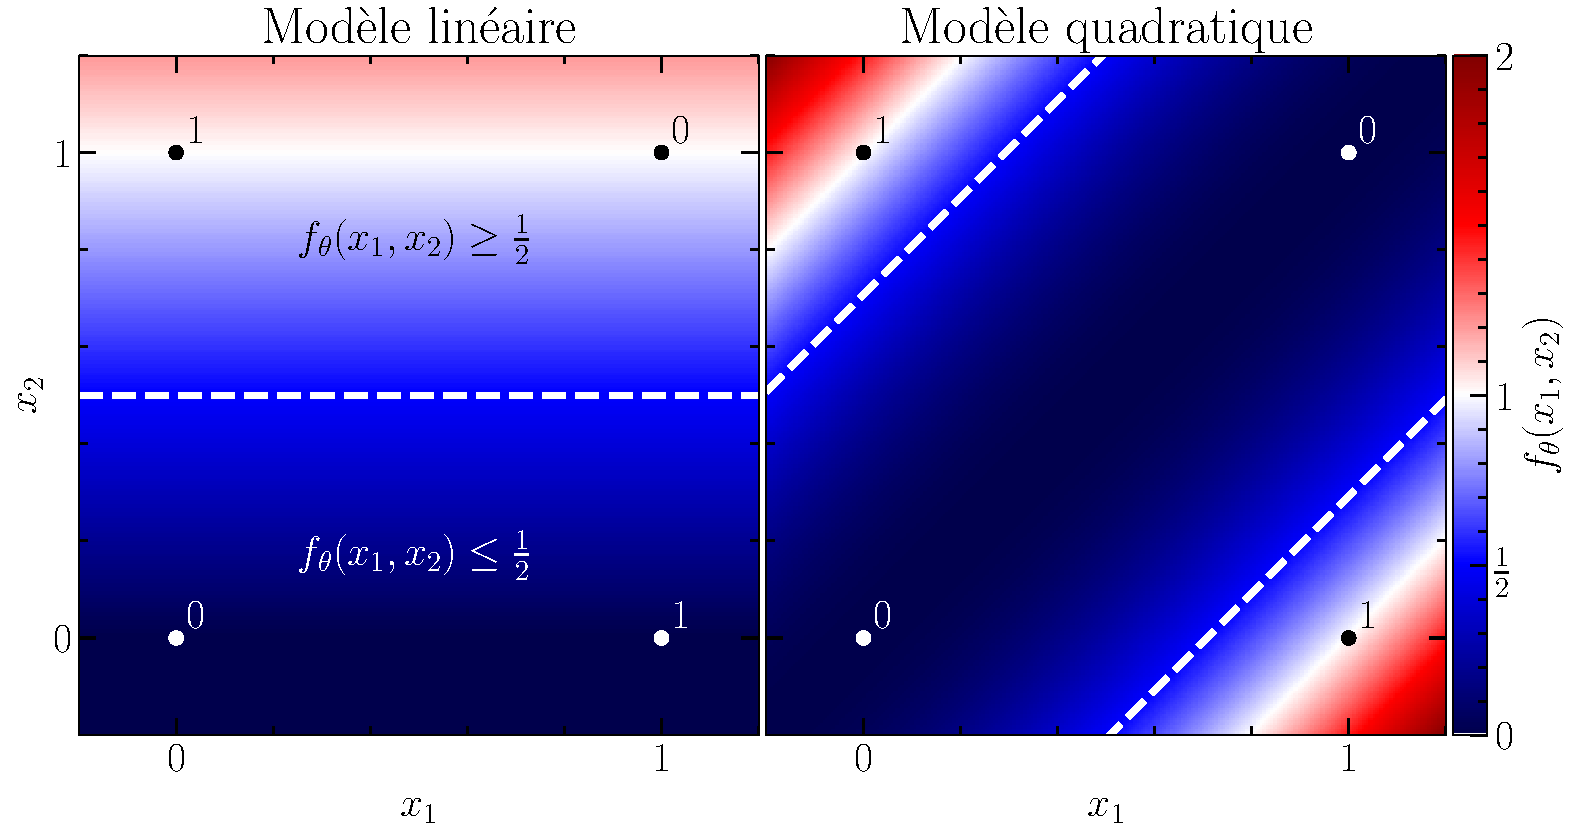
\includegraphics[width=0.7\textwidth]{notebooks/xor.pdf}
        \caption{Comparaison d'un modèle linéaire et d'un modèle quadratique pour le problème XOR.}
        \label{fig:xor}
\end{figure}

Malgré cela, on peut explorer l'application d'un modèle comme \eqref{eq:multidim expansion} dans le but de développer 
une intuition géométrique qui servira à introduire la prochaine méthode pour complexifier $f_\theta$.
On considère l'exemple le plus simple qui requiert un modèle quadratique, 
soit la fonction logique OU exclusive (mieux connue comme XOR dans le jargon de la science informatique). Cette fonction logique peut être 
décrite de façon exhaustive avec la table \ref{tab:xor}.
\begin{table}[ht!]
        \centering
        \begin{tabular}{ccc}
                $x_1$ & $x_2$ & $f_{\theta^{\star}}(x_1, x_2)$  \\\hline
                0 & 0 & 0 \\ 
                0 & 1 & 1 \\
                1 & 0 & 1 \\
                1 & 1 & 0 \\\hline
        \end{tabular}
        \caption{Fonction logique XOR.}
        \label{tab:xor}
\end{table}


%Un ajustement de paramètres d'une fonction linéaire
Ce problème ne peut pas être résolu par une fonction linéaire puisque les 4 contraintes du problème ne sont pas linéairement séparables.
Plus spécifiquement, on ne peut pas construire de plan qui sépare les points qui correspondent à $f_{\theta^{\star}} = 0$ des points 
qui correspondent à $f_{\theta^{\star}} = 1$. Le panneau gauche de la figure \ref{fig:xor} montre le modèle linéaire
\begin{equation}\label{eq:sol1}
        f_{\hat{\theta}}(x_1, x_2) = \begin{bmatrix}0 & 1 \end{bmatrix} \begin{bmatrix} x_1 \\ x_2 \end{bmatrix} = x_2\, 
\end{equation}
pour illustrer cet argument. 
Ce fait est saillant dans le panneau gauche de la figure \ref{fig:xor}, où on montre comment le plan $f_{\hat{\theta}}(x_1, x_2) = \frac{1}{2}$ (ligne pointillée blanche) 
n'est pas en mesure de séparer les 4 contraintes linéairement.
De plus, aucune rotation ou translation (et en général aucune transformation affine) de ce modèle 
ne peut séparer les points $0$ et $1$ linéairement. 
Ainsi, ce modèle est optimal, mais pas unique, en termes du nombre de contraintes retrouvées. On conclut que l'ensemble des modèles linéaires ne contient pas 
la fonction XOR.
%On notera que le modèle n'est pas optimal en termes de l'erreur moyenne quadratique puisque $f_\theta(x_1, x_2) = \frac{1}{2}$ possède une erreur inférieure (et optimale), 
%bien que ce dernier ne recouvre aucune contrainte. 

Pour résoudre le problème, on doit introduire le terme de second degré dans la série de puissances \eqref{eq:multidim expansion}. 
Cet ensemble de fonctions contient une infinité de solutions au problème XOR. Le panneau de droite de la figure \ref{fig:xor} 
illustre la solution particulière
\begin{equation}\label{eq:sol quad}
        f_{\hat{\theta}}(x_1, x_2) = \begin{bmatrix} x_1 & x_2 \end{bmatrix} \begin{bmatrix} 1 & -1 \\ -1 & 1 \end{bmatrix} \begin{bmatrix} x_1 \\ x_2 \end{bmatrix} = (x_1 - x_2)^2\,
\end{equation} 
qui recouvre parfaitement les 4 contraintes du problème XOR. Il est intéressant de noter que 
cette solution possède une quantité caractéristique, $h = (x_1 - x_2)^2$, qui est linéairement séparable. En effet, 
on peut tracer un plan $h = \frac{1}{2}$ qui sépare les points $0$ et $1$ dans cet espace. 

Cette observation motive l'introduction d'une nouvelle méthode pour complexifier notre modèle. 
Cette méthode devrait minimalement être en mesure de construire un espace caractéristique (de l'anglais \textit{feature space}) 
équivalent à $h = (x_1 - x_2)^2$, soit un espace caractéristique où les contraintes d'un problème donné sont linéairement séparables.
C'est cette quête qui nous mène naturellement à l'apprentissage profond. 


\section{Les réseaux de neurones}\label{sec:app profond}

Les réseaux de neurones ont été introduits par \citet{Rosenblatt1958} comme des circuits analogues à des circuits biologiques 
de neurones. L'espoir était de mieux comprendre comment les systèmes biologiques sont en mesure de percevoir 
leur environnement; comment l'information est apprise, préservée, remémorée et finalement comment ces systèmes sont 
en mesure de réfléchir, soit prendre en compte toute l'information à leur disposition (perception et mémoire) 
pour dicter ou influencer un comportement. Il s'avère toutefois que ces circuits ont des propriétés qui les rend 
particulièrement intéressants dans le contexte de l'apprentissage machine. 
Ce sont ces propriétés qui nous concernent dans cette section.

\begin{figure}[H]
 \centering
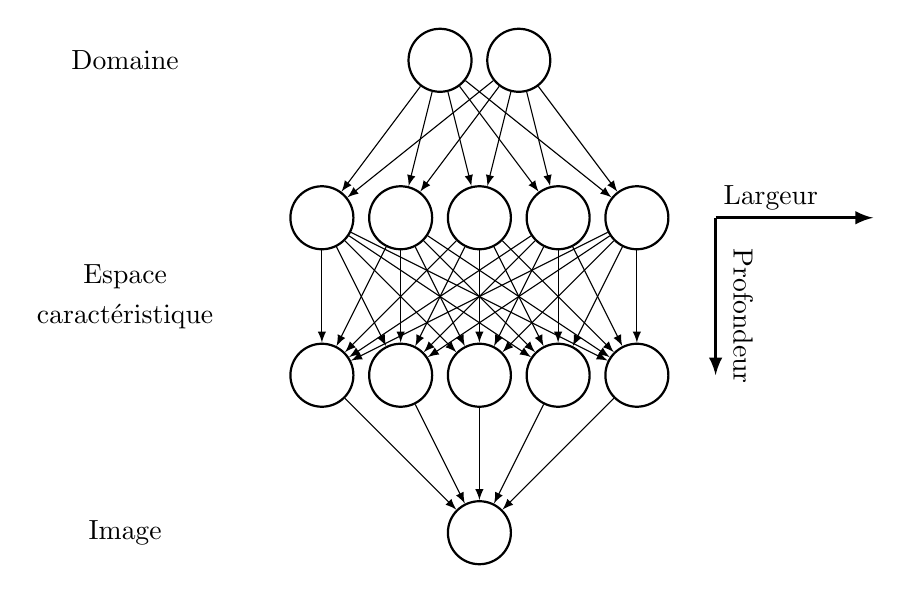
\begin{tikzpicture}
\tikzset{cnode/.style={circle, draw=black, thick, minimum size=0.8cm}}
\node at (-4, 0) {Domaine};
\foreach \i in {0,...,1}
{
        \node[cnode] (x\i) at (\i, 0) {};
}
\node at (-4, -2.75) {Espace};
\node at (-4, -3.25) {caractéristique};

\node at (4.2, -1.75) {Largeur};
\node[rotate=-90] at (3.85, -3.25) {Profondeur};
\draw[-latex, very thick] (3.5, -2) -- (3.5, -4);
\draw[-latex, very thick] (3.5, -2) -- (5.5, -2);
\foreach \i in {0,...,4}
{
        \node[cnode] (z\i) at (\i-1.5, -2) {};
}
\foreach \i in {0,...,4}
{
        \node[cnode] (h\i) at (\i-1.5, -4) {};
}
\node at (-4, -6) {Image};
\node[cnode] (y) at (0.5, -6) {};
\foreach \i in {0,...,1}
{
        \foreach \j in {0,...,4}
        {
                \draw[-latex, thin] (x\i) to (z\j);
        }
}
\foreach \i in {0,...,4}
{
        \foreach \j in {0,...,4}
        {
                \draw[-latex, thin] (z\i) to (h\j);
        }
}
\foreach \j in {0,...,4}
{
        \draw[-latex, thin] (h\j) to (y);
}
\end{tikzpicture}
\caption{Illustration d'un réseau de neurones avec deux couches latentes qui constituent son espace caractéristique.}
\label{fig:mlp}
\end{figure}

La structure mathématique d'un réseau de neurones est généralement introduite à l'aide d'un graphe acyclique, 
tels qu'illustré à la figure \ref{fig:mlp}. Une description tout à fait équivalente de ces réseaux est la  
composition de fonctions
\begin{equation}\label{eq:composition}
        f_\theta(\mathbf{x}) = (f^{(P)}_\theta \circ f^{(P-1)}_\theta \circ \dots \circ f^{(1)}_\theta)(\mathbf{x})\, .
\end{equation} 
Les couches du réseau (de l'anglais \textit{layer}), $f_\theta^{(i)}: \mathbb{R}^{n} \rightarrow \mathbb{R}^{m}$, sont formées de deux composantes essentielles, 
soit une transformation affine $\mathbf{W}\mathbf{z} + \mathbf{b}$ et une fonction non linéaire $\sigma: \mathbb{R} \rightarrow  \mathbb{R}$ 
(aussi appelée fonction d'activation)
\begin{equation}\label{eq:mlp layer}
        f^{(i)}_\theta(\mathbf{z}) = \sigma( \mathbf{W}^{(i)} \mathbf{z} + \mathbf{b}^{(i)})\, .
\end{equation} 
On note $\mathbf{W} \in \mathbb{R}^{m \times n}$, une matrice de poids (de l'anglais \textit{weights}), et 
$\mathbf{b} \in \mathbb{R}^{m}$, un vecteur de biais (de l'anglais \textit{bias}, à ne pas confondre avec le biais statistique mentionné précédemment). 
Dans cette expression, il est sous-entendu que la fonction 
d'activation, $\sigma$, s'applique identiquement sur les $m$ éléments du vecteur $\mathbf{W} \mathbf{z} + \mathbf{b}$. 

Séparées, la transformation affine et la fonction d'activation ne sont pas en mesure de résoudre des problèmes comme XOR. En effet, 
une transformation affine préserve les lignes parallèles d'un espace vectoriel, de sorte 
qu'un ensemble de points qui n'est pas linéairement séparable le restera après une transformation affine. 
D'un autre côté, comme une fonction d'activation agit directement sur les coordonnées, ce type de fonction n'est 
pas en mesure de construire une quantité caractéristique qui mélange les coordonnées 
comme celle trouvée à la section précédente, $h = (x_1 - x_2)^{2}$. 

C'est l'application combinée de ces deux ingrédients qui permet minimalement de résoudre un problème comme XOR. Par exemple, 
considérons la fonction d'activation traditionnelle $\mathrm{ReLU}$ (inspiré des neurones biologiques)
\begin{equation}
        \mathrm{ReLU}(x) = 
        \begin{cases}
                x & x \geq 0 \\
                0 & x < 0
        \end{cases}
        =
        \max(0, x), \hspace{1cm} x \in \mathbb{R}
\end{equation}
Pour résoudre le problème XOR, on introduit une seule couche cachée dans le réseau de neurones
\begin{equation}
        f_\theta = \mathbf{w}(f^{(1)}_\theta(\mathbf{x})) + \mathbf{b}\, .
\end{equation} 
La dernière couche du réseau est une transformation affine, puisqu'on s'attend à ce que la couche cachée $f^{(1)}_\theta$ puisse 
construire un espace caractéristique qui sépare linéairement les contraintes du problème. Il s'avère que cette construction 
admet la solution suivante
\begin{equation}\label{eq:sol2}
        f_{\hat{\theta}}(x_1, x_2) =
        \begin{bmatrix}
                1 & 1 
        \end{bmatrix}
        \mathrm{ReLU}\left(  
        \begin{bmatrix}
        1 & -1 \\ -1 & 1     
        \end{bmatrix}
        \begin{bmatrix}
                x_1 \\ x_2
        \end{bmatrix}
        \right)
        = \max(0,\, x_1 - x_2) + \max(0,\, x_2 - x_1)\, ,
\end{equation}
où la transformation affine de la couche cachée est la même que celle trouvée dans la section précédente. Pour comprendre intuitivement 
le rôle de chaque composante de ce réseau, la figure \ref{fig:xor2} illustre comment les opérations séquentielles du réseau de neurones \eqref{eq:sol2} 
transforment l'espace du problème vers un espace caractéristique linéairement séparable (identifiable par une droite pointillée).

\begin{figure}[ht!]
\centering
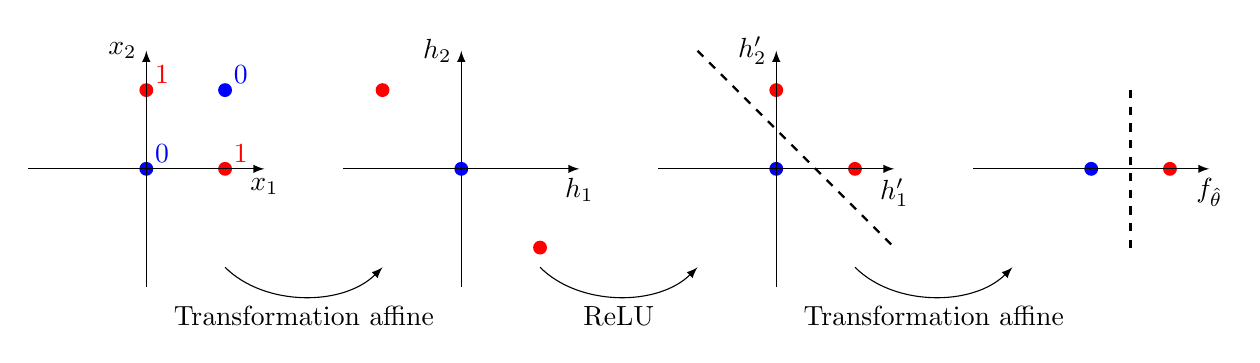
\begin{tikzpicture}
\begin{scope}[shift={(-4,0)}]
        \node[circle, fill=blue, minimum size=5pt, inner sep=0pt] at (1, 1) {};
        \node[circle, fill=blue, minimum size=5pt, inner sep=0pt] at (0, 0) {};
        \node[circle, fill=red, minimum size=5pt, inner sep=0pt] at (0, 1) {};
        \node[circle, fill=red, minimum size=5pt, inner sep=0pt] at (1, 0) {};
        \node[color=red] at (1.2, .2) {$1$};
        \node[color=blue] at (1.2, 1.2) {$0$};
        \node[color=red] at (.2, 1.2) {$1$};
        \node[color=blue] at (.2, .2) {$0$};
        \draw[-latex] (0, -1.5) -- (0, 1.5) node[at end, left] {$x_2$};
        \draw[-latex] (-1.5, 0) -- (1.5, 0) node[at end, below] {$x_1$};
\end{scope}
\draw[-latex] (-3, -1.25) .. controls +(.5, -.5) and +(-.5, -.5) .. (-1, -1.25) node[below, midway] {Transformation affine};

\begin{scope}[shift={(0,0)}]
        \node[circle, fill=red, minimum size=5pt, inner sep=0pt] at (1, -1) {};
        \node[circle, fill=blue, minimum size=5pt, inner sep=0pt] at (0, 0) {};
        \node[circle, fill=red, minimum size=5pt, inner sep=0pt] at (-1, 1) {};
        \draw[-latex] (0, -1.5) -- (0, 1.5) node[at end, left] {$h_2$};
        \draw[-latex] (-1.5, 0) -- (1.5, 0) node[at end, below] {$h_1$};
\end{scope}
\draw[-latex] (1, -1.25) .. controls +(.5, -.5) and +(-.5, -.5) .. (3, -1.25) node[below, midway] {ReLU};

\begin{scope}[shift={(4,0)}]
        \node[circle, fill=red, minimum size=5pt, inner sep=0pt] at (1, 0) {};
        \node[circle, fill=blue, minimum size=5pt, inner sep=0pt] at (0, 0) {};
        \node[circle, fill=red, minimum size=5pt, inner sep=0pt] at (0, 1) {};
        \draw[-latex] (0, -1.5) -- (0, 1.5) node[at end, left] {$h'_2$};
        \draw[-latex] (-1.5, 0) -- (1.5, 0) node[at end, below] {$h'_1$};
        \draw[dashed, thick] (-1, 1.5) -- (1.5, -1);
\end{scope}

\draw[-latex] (5, -1.25) .. controls +(.5, -.5) and +(-.5, -.5) .. (7, -1.25) node[below, midway] {Transformation affine};

\begin{scope}[shift={(8,0)}]
        \node[circle, fill=red, minimum size=5pt, inner sep=0pt] at (1, 0) {};
        \node[circle, fill=blue, minimum size=5pt, inner sep=0pt] at (0, 0) {};
        \draw[-latex] (-1.5, 0) -- (1.5, 0) node[at end, below] {$f_{\hat{\theta}}$};
        \draw[dashed, thick] (0.5, 1) -- (0.5, -1);
\end{scope}
        
\end{tikzpicture}
\caption{Illustration d'une transformation du problème XOR vers un espace caractéristique linéairement séparable par un réseau de neurones.}
\label{fig:xor2}
\end{figure}

L'espace caractéristique des réseaux de neurones est la source de leur flexibilité. Le théorème d'approximation universel 
\citep{Cybenko1989,Hornik1991} stipule 
qu'un réseau avec une seule couche cachée d'une largeur suffisante (dimension de l'espace caractéristique) peut représenter 
n'importe quelle fonction continue.
Il est possible d'obtenir une limite supérieur pour la largeur du réseau de neurones par des arguments géométriques dans des cas simples comme XOR.
En général, un problème de classification binaire avec $N$ points de données (4 dans le cas de XOR) est toujours linéairement séparable dans 
un espace caractéristique de dimensions $D$ tels que $D \geq N - 1$. 

Ce critère provient du théorème de \citet{Cover1965} et de la dimension de Vapnik-Chervonenkis d'un classificateur linéaire \citep{Vapnik1971,Vapnik1995}. 
La probabilité qu'un ensemble de $N$ points soit linéairement séparable augmente 
considérablement en fonction de la dimension de l'espace, et atteint $p = 1$ lorsque $D \geq N -1$.
Pour le problème XOR, on a trouvé que $D=2$ admettait une solution. 
%En général, le théorème de Cover est une limite supérieure sur la dimensionnalité de l'espace caractéristique, 
%et garantit qu'un réseau de neurones à une couche peut résoudre un problème de classification binaire arbitrairement complexe. 
Il est assez rare que cette limite supérieure soit 
atteinte puisque les données réelles tendent à se regrouper sur des variétés de basses dimensions. 
Par contre, spécifier une couche cachée suffisamment large peut devenir rapidement intraitable dans certaines situations, 
particulièrement en hautes dimensions. C'est un problème similaire à celui rencontré à la section précédente avec la série entière. 
La prochaine section introduira certaines stratégies pour contourner ce problème.

Finalement, on doit mentionner que les réseaux de neurones 
ne sont pas des fonctions linéaires en fonction de leurs paramètres (contrairement à la série entière). 
Ainsi, l'apprentissage profond introduit un problème d'optimisation non linéaire, soit un problème avec 
potentiellement plusieurs minimas secondaires et une géométrie non triviale.
Les algorithmes d'apprentissage modernes
sont largement équipés pour résoudre ce genre de problème grâce à l'introduction des dérivées automatiques et 
des algorithmes de descente de gradient stochastiques. Voir le livre de référence de \citet{Goodfellow2016} 
pour une discussion plus détaillée de ce sujet.

Je termine finalement ce chapitre avec une très courte introduction sur les réseaux neuronaux convolutifs. Ces réseaux sont utilisés 
extensivement dans les deux prochains chapitres étant donné que le problème étudié dans ce mémoire nécessite l'introduction de réseaux 
spécialisés pour le traitement d'image. 

\section{Les réseaux de neurones convolutifs}\label{sec:cnn}
Le traitement d'image pose un problème sérieux à l'apprentissage machine en raison de la dimensionalité du problème. 
Une image est généralement décrite par 3 dimensions qui décrivent respectivement la hauteur ($H$), la largeur ($L$) et le nombre de canaux de couleurs ($C$). 
La dimensionalité d'une image correspond au nombre total de pixels qui décrivent cette image, soit $C \times H \times L $, 
un nombre qui peut facilement atteindre une valeur de l'ordre de $\mathcal{O}(10^{5})$ en astronomie.

Pour construire une fonction avec un nombre raisonnable de paramètres, on utilise le principe d'équivarience. 
Ce principe est fortement inspiré du principe de la covariance, originellement formulé 
par Einstein, qui stipule qu'une théorie physique devrait être formulée en termes des quantités qui se transforme de façon covariantes 
par rapport à une action du groupe de symétrie de la théorie. Le principe d'équivarience stipule similairement qu'une fonction $f_\theta$ doit se transformer de façon équivariente
sous l'action du groupe de symétrie $G$ du problème à l'étude
\begin{equation}
        \begin{split}
                x &\rightarrow Tx\\
                f_\theta(x) &\rightarrow f'_\theta(Tx) = T'f_\theta(x) \, .
        \end{split}
\end{equation} 
$T, T' \in G$ sont des éléments du groupe de symétrie. $T'$ est la représentation de l'action $T$ dans l'espace vectoriel de l'image de la fonction $f_\theta$.

La convolution est une opération équivariante sous l'effet d'une translation. 
Pour rendre cette observation concrète, prenons l'exemple de la convolution entre le noyau de la convolution $\mathbf{W} \in \mathbb{R}^{m}$ 
et un vecteur $\mathbf{x} \in \mathbb{R}^{n}$
\begin{equation}\label{eq:conv}
        (\mathbf{W} * \mathbf{x})_j = \sum_{i = 0}^{m-1} \mathbf{W}_i\, \mathbf{x}_{j - i}
\end{equation} 
L'effet d'une translation sur le vecteur $\mathbf{x}$ est de modifier l'ordre des indices. On note $T_{w}$ une translation 
qui déplace les indices de la façon suivante $T_w\mathbf{x}_{j} = \mathbf{x}_{j+w}$. Il est sous-entendu que les indices sont définis $\mathrm{mod}\, n$. 
On peut alors montrer que la convolution \eqref{eq:conv} est une opération équivariante sous l'effet d'une translation 
\begin{equation}
        (\mathbf{W} *(T_w\mathbf{x}))_j = \sum_{i = 0}^{m-1} \mathbf{W}_i\, \mathbf{x}_{j + w - i} = (\mathbf{W} * \mathbf{x})_{j + w} = T_w(\mathbf{W} * \mathbf{x})_{j}
\end{equation} 
Comparé à une transformation affine, le noyau de la convolution requiert beaucoup moins de paramètres pour un niveau comparable d'expressivité. En effet, 
il est souvent justifié de supposer que l'information à extraire du domaine est localement corrélée. 
En supposant que la distance de corrélation est $m< n$, on peut construire un noyau pour la convolution avec $m$ paramètres. C'est un énorme  
avantage comparé à la transformation affine. Cette dernière a besoin, minimalement, de $n$ paramètres pour chaque dimension 
de l'espace caractéristique.

Cet avantage devient significatif lorsqu'on considère des images $\mathbf{x} \in \mathbb{R}^{C \times H\times L}$, soit des tenseurs de rang 3. 
On considère une convolution sur les dimensions spatiales seulement ($H$ et $L$) et on pose ${W \in \mathbb{R}^{C \times c \times h \times \ell }}$. On définit la convolution sur une image 
\begin{equation}
        (\mathbf{W} * \mathbf{x})_{ijk} = \sum_{m=0}^{C-1} \sum_{n=0}^{h-1}\sum_{p=0}^{\ell-1}\mathbf{W}_{minp} \mathbf{x}_{m,j-n,k-p}
\end{equation} 
Les dimensions spatiales du noyau sont généralement choisis tels que $h \ll H$ et $\ell \ll L$ 
puisque l'information pertinente est locale pour les tâches de traitement d'images typiques. Par 
exemple, taille du noyau $h = \ell = 3 $ est choix commun même lorsque la taille d'une image atteint $H \times L \gtrsim 10^4$. L'expressivité d'un réseau de neurones 
convolutifs \citep{LeCun1995} dépend principalement du nombre de canaux utilisés pour l'espace caractéristique 
et de la profondeur du réseau \citep{Krizhevsky2012}.

Ceci complète donc cette introduction à l'apprentissage machine. Comme l'architecture des réseaux 
de neurones est un sujet qui dépend du problème à l'étude, ce sujet est abordé dans 
les prochains chapitres qui traitent en détails des méthodes utilisées dans ce mémoire.

